
%(BEGIN_QUESTION)
% Copyright 2010, Tony R. Kuphaldt, released under the Creative Commons Attribution License (v 1.0)
% This means you may do almost anything with this work of mine, so long as you give me proper credit

Suppose we have an Allen-Bradley model ``SLC 500'' PLC connected to a pair of pushbutton switches and light bulbs as shown in this illustration:

$$\includegraphics[width=15.5cm]{i04629x01.eps}$$

Examine the following relay ladder logic (RLL) program for this Allen-Bradley PLC, determining the necessary switch statuses to energize lamp Y, and the necessary switch statuses to energize switch Z:

$$\includegraphics[width=15.5cm]{i04629x02.eps}$$

\underbar{file i04629}
%(END_QUESTION)





%(BEGIN_ANSWER)

To energize lamp Z: {\bf press} switch B, {\bf release} switch A.

\vskip 10pt

To energize lamp Y: {\bf press} switch A, {\bf release} switch B.

%(END_ANSWER)





%(BEGIN_NOTES)


%INDEX% PLC, relating I/O status to virtual elements

%(END_NOTES)


